\documentclass{article}

\usepackage{arxiv}

\usepackage[utf8]{inputenc} % allow utf-8 input
\usepackage[T1]{fontenc}    % use 8-bit T1 fonts
\usepackage{lmodern}        % https://github.com/rstudio/rticles/issues/343
\usepackage{hyperref}       % hyperlinks
\usepackage{url}            % simple URL typesetting
\usepackage{booktabs}       % professional-quality tables
\usepackage{amsfonts}       % blackboard math symbols
\usepackage{nicefrac}       % compact symbols for 1/2, etc.
\usepackage{microtype}      % microtypography
\usepackage{graphicx}

\title{Reproducible and Programmatic Generation of Neuroimaging Visualizations}

\author{
    Sidhant Chopra
    \thanks{Corresponding author}
   \\
    Department of Psychology \\
    Yale University \\
  CT, USA, 06511 \\
  \texttt{\href{mailto:sidhant.chopra@yale.com}{\nolinkurl{sidhant.chopra@yale.com}}} \\
   \And
    Loïc Labache
   \\
    Department of Psychology \\
    Yale University \\
  CT, USA, 06511 \\
  \texttt{} \\
   \And
    Elvisha Dhamala
   \\
    Department of Psychology \\
    Yale University \\
  CT, USA, 06511 \\
  \texttt{} \\
   \And
    Edwina R Orchard
   \\
    Department of Psychology \\
    Yale University \\
  CT, USA, 06511 \\
  \texttt{} \\
   \And
    Avram Holmes
   \\
    Department of Psychology \\
    Yale University \\
  CT, USA, 06511 \\
  \texttt{} \\
  }

% Pandoc syntax highlighting
\usepackage{color}
\usepackage{fancyvrb}
\newcommand{\VerbBar}{|}
\newcommand{\VERB}{\Verb[commandchars=\\\{\}]}
\DefineVerbatimEnvironment{Highlighting}{Verbatim}{commandchars=\\\{\}}
% Add ',fontsize=\small' for more characters per line
\usepackage{framed}
\definecolor{shadecolor}{RGB}{248,248,248}
\newenvironment{Shaded}{\begin{snugshade}}{\end{snugshade}}
\newcommand{\AlertTok}[1]{\textcolor[rgb]{0.94,0.16,0.16}{#1}}
\newcommand{\AnnotationTok}[1]{\textcolor[rgb]{0.56,0.35,0.01}{\textbf{\textit{#1}}}}
\newcommand{\AttributeTok}[1]{\textcolor[rgb]{0.77,0.63,0.00}{#1}}
\newcommand{\BaseNTok}[1]{\textcolor[rgb]{0.00,0.00,0.81}{#1}}
\newcommand{\BuiltInTok}[1]{#1}
\newcommand{\CharTok}[1]{\textcolor[rgb]{0.31,0.60,0.02}{#1}}
\newcommand{\CommentTok}[1]{\textcolor[rgb]{0.56,0.35,0.01}{\textit{#1}}}
\newcommand{\CommentVarTok}[1]{\textcolor[rgb]{0.56,0.35,0.01}{\textbf{\textit{#1}}}}
\newcommand{\ConstantTok}[1]{\textcolor[rgb]{0.00,0.00,0.00}{#1}}
\newcommand{\ControlFlowTok}[1]{\textcolor[rgb]{0.13,0.29,0.53}{\textbf{#1}}}
\newcommand{\DataTypeTok}[1]{\textcolor[rgb]{0.13,0.29,0.53}{#1}}
\newcommand{\DecValTok}[1]{\textcolor[rgb]{0.00,0.00,0.81}{#1}}
\newcommand{\DocumentationTok}[1]{\textcolor[rgb]{0.56,0.35,0.01}{\textbf{\textit{#1}}}}
\newcommand{\ErrorTok}[1]{\textcolor[rgb]{0.64,0.00,0.00}{\textbf{#1}}}
\newcommand{\ExtensionTok}[1]{#1}
\newcommand{\FloatTok}[1]{\textcolor[rgb]{0.00,0.00,0.81}{#1}}
\newcommand{\FunctionTok}[1]{\textcolor[rgb]{0.00,0.00,0.00}{#1}}
\newcommand{\ImportTok}[1]{#1}
\newcommand{\InformationTok}[1]{\textcolor[rgb]{0.56,0.35,0.01}{\textbf{\textit{#1}}}}
\newcommand{\KeywordTok}[1]{\textcolor[rgb]{0.13,0.29,0.53}{\textbf{#1}}}
\newcommand{\NormalTok}[1]{#1}
\newcommand{\OperatorTok}[1]{\textcolor[rgb]{0.81,0.36,0.00}{\textbf{#1}}}
\newcommand{\OtherTok}[1]{\textcolor[rgb]{0.56,0.35,0.01}{#1}}
\newcommand{\PreprocessorTok}[1]{\textcolor[rgb]{0.56,0.35,0.01}{\textit{#1}}}
\newcommand{\RegionMarkerTok}[1]{#1}
\newcommand{\SpecialCharTok}[1]{\textcolor[rgb]{0.00,0.00,0.00}{#1}}
\newcommand{\SpecialStringTok}[1]{\textcolor[rgb]{0.31,0.60,0.02}{#1}}
\newcommand{\StringTok}[1]{\textcolor[rgb]{0.31,0.60,0.02}{#1}}
\newcommand{\VariableTok}[1]{\textcolor[rgb]{0.00,0.00,0.00}{#1}}
\newcommand{\VerbatimStringTok}[1]{\textcolor[rgb]{0.31,0.60,0.02}{#1}}
\newcommand{\WarningTok}[1]{\textcolor[rgb]{0.56,0.35,0.01}{\textbf{\textit{#1}}}}

% tightlist command for lists without linebreak
\providecommand{\tightlist}{%
  \setlength{\itemsep}{0pt}\setlength{\parskip}{0pt}}

% From pandoc table feature
\usepackage{longtable,booktabs,array}
\usepackage{calc} % for calculating minipage widths
% Correct order of tables after \paragraph or \subparagraph
\usepackage{etoolbox}
\makeatletter
\patchcmd\longtable{\par}{\if@noskipsec\mbox{}\fi\par}{}{}
\makeatother
% Allow footnotes in longtable head/foot
\IfFileExists{footnotehyper.sty}{\usepackage{footnotehyper}}{\usepackage{footnote}}
\makesavenoteenv{longtable}


\usepackage{pdflscape}
\newcommand{\blandscape}{\begin{landscape}}
\newcommand{\elandscape}{\end{landscape}}
\usepackage{setspace}\doublespacing
\begin{document}
\maketitle


\begin{abstract}
Neuroimaging visualization forms the centrepiece of quality control, and interpretation and communication of results. Often, these images and figures are produced by manually changing settings on Graphical User Interfaces (GUI). There now exist many well-documented code-based brain visualisation tools that allow users to programmatically generate publication-ready figures directly within environments such as R, Python and MATLAB. Compared to figures generated using GUIs, programmatic tools are more replicable, flexible, interactive, and integrated with the scientific process. This article reviews the advantages of learning and using programmatic neuroimaging visualization tools and provides a list of tools across programming environments. Finally, we introduce examples of specific R and Python tools for visualization of voxel, vertex, region-of-interest, and edge level data.
\end{abstract}

\keywords{
    Neuroimaging visualization
   \and
    Reproducibility
   \and
    Programmatic figures
   \and
    Open Science
   \and
    R
   \and
    Python
   \and
    Brain Visualization
  }

\hypertarget{introduction}{%
\section{Introduction}\label{introduction}}

The visualization of neuroimaging data is one of the primary ways in which we evaluate data quality, interpret results, and communicate findings. These visualizations are commonly produced using graphical user interface-based (GUI) tools where individual images are opened and, within each instance, display settings are manually changed until the desired output is reached. In large part, the choice to use GUI-based software has been driven by a perception of convenience, flexibility, and accessibility. However, there now exists many code-based software packages which are well-documented and often do not require high-level knowledge of programming, making them more accessible to the neuroimaging community (Table 1). These tools are flexible and allow for the generation of reproducible, high-quality, and publication-ready brain visualizations in only a few lines of code (Figure 1), especially within the R, Python and MATLAB environments.

The present article covers three major advantages of using code-generated visualizations over GUI based tools: replicability, flexibility, and integration. First, by generating visualizations using code, you increase the replicability of your figures for yourself, your collaborators and your readers. Second, code-based tools provides more precise controls over display settings, while also benefiting from the advantages of programming, such as the ability to iteratively and rapidly generate multiple figures. Finally, being able to integrate figure generation into your analysis scripts reduces chances of errors and increases the accessibility of resulting analyses pipeline, with more advanced tools now allowing for the seamless integration of prose and code. Here, we review the advantages of learning and using programmatic neuroimaging visualizations, focusing on benefits to replicability, flexibility and integration. We conclude by introducing examples of R-packages which allow for visualization of statistics at region-of-interest (ROI), voxel, vertex, and edge level data, followed by a brief discussion of limitations and functionality gaps in code-based brain visualization tools.

\hypertarget{replicability}{%
\section{Replicability}\label{replicability}}

In recent years, there have been multiple large-scale efforts empirically demonstrating the lack of reproducibility of findings from neuroimaging data (Poldrack et al., 2017). One common solution proposed for achieving robust and reliable discoveries has been to encourage scientific output which can be transparently evaluated and independently replicated. In practice, this typically entails openly sharing detailed methods, materials, code, and data. While there is a trend towards increasing transparency and code sharing of neuroimaging analyses, the sharing of code used to generate figures which include brain renderings and spatial maps has been relatively neglected. This gap in reproducibility is partly driven by the fact that brain figures are often created using a manual process that involves tinkering with sliders, buttons, and overlays on a GUI, concluding with a screenshot and sometimes beautification in image processing software like Illustrator or Photoshop. Such a process inherently makes neuroimaging visualizations difficult, if not impossible to replicate, even by the authors themselves.

Visualization scripts should reflect a core feature of open science. Given that brain figures regularly form the centerpiece of interpretation within papers, conference presentations, or news reports, making sure they can be reliably regenerated is crucial for knowledge generation. By writing and sharing code used to generate brain visualizations, a direct and traceable link is established between the underlying data and the corresponding scientific figure. While the code that produces a replicable figure doesn't necessarily reflect the validity of the scientific finding or the accuracy of the associated content, it allows for reproducibility, instilling transparency and robustness, while demonstrating a desire to further scientific knowledge. Some even consider publishing figures which cannot be replicated as closer to advertising, rather than science (Steel, 2013).

While some GUI-based tools have historically offered command-line access to generate replicable visualizations, they can lack both the flexibility to easily generate publication ready figures and the benefits, such as iteration, provided by your preferred programming environment. Likewise, other GUI-based tools offer replicability in the form of automatically generated batch scripts or in-built terminals, which are often idiosyncratic and lack documentation to make them easily usable or reproducible by those not familiar with the specific software.

\hypertarget{flexibility}{%
\section{Flexibility}\label{flexibility}}

Being able to exactly replicate your figures via code has marked advantages beyond positive open science practices. In particular, the ability to reprogram inputs (such as statistical maps) and settings (such as color schemes, thresholds, and visual orientations) can streamline your entire scientific workflow. Changing inputs and settings via code allows for the easy production of multiple figures, such as those resulting from multiple analyses which require similar visualizations. A simple for-loop or copying and pasting the code with altered input and/or settings-of-interest can be a powerful method for exploring visualization options or rapidly creating multi-panel figures. Likewise, an arduous request from a reviewer or collaborator to alter the image processing or analysis becomes less of a burden when the associated figures can be re-generated with a few lines of code, as opposed to re-pasting and re-illustrating them manually. Having a code-base with modifiable inputs can mean that the generation of visualizations requires less time, energy and effort than image and instance specific GUI-based generation. This also makes it easier to generate consistent figures across subsequent projects. Keep in mind that the gains of writing code for your figures are cumulative, and in addition to improving your programming, you start to build a code-base for figure generation that you can continue to reuse and share throughout your scientific career.

Precise controls via code over visualization settings, such as color schemes, legend placement and camera angles, can provide you with much greater flexibility over visualizations. Nonetheless, part of the appeal of GUI-based tools is that the presets for such settings can provide a useful starting point and reduce the decision burden on novice users. However, similar presets are often available in the form of default settings across most code-based packages, negating the need for the user to manually enter each and every choice of setting required for creating an image. Most code-based tools also come with documentation, with R-packages on the \emph{CRAN} or \emph{Neuroconductor} (Muschelli et al., 2019) repositories requiring detailed guidance. Recent packages have started to include detailed documentation in GitHub repositories, or even entire papers (e.g., Pham, Muschelli, \& Mejia, 2022; Mowinckel \& Vidal-Piñeiro, 2020; Huntenburg et at., 2017; Schäfer \& Ecker, 2020) which provide examples of figures that can be used as starting points or templates for new users. As the popularity of code-sharing for figure increases, there will be a cornucopia of templates that can be used as the basis for new figures.

While brain visualizations are often thought of as the end results of analyses, they also form a vital part of quality control for imaging data. Tools to automatically detect artefacts, de-noise the data and generate derivatives are becoming more robust, but we are not yet at the stage where visualizing the data during processing is no longer necessary. Nonetheless, when working with large datasets such as Human Connectome Project (Van Essen et al., 2013) or UK BioBank (Sudlow et al., 2015), it is unfeasible to use traditional GUI-based tool to visually examine the data. The time it takes to open a single file and achieve the desired visualization settings vastly compounds when working with large datasets. Knowing how to programmatically generate brain visualizations can allow you to iterate your visualization code over each image of a large datasets making checking the quality of each data processing or analysis step accessible and achievable. The visual outputs of each iteration can be complied into accessible documents which can be easily scrolled, with more advanced usage allowing for the creation of interactive HTML reports, similar to those created by standardized data processing tools like \emph{fmriprep} (Esteban et al., 2019). Increasing capacity to conduct visual quality control on larger datasets can increase the identification of processing errors and result in more reliable and valid findings from your data.

\hypertarget{integrative-and-interactive-reporting}{%
\section{Integrative and Interactive Reporting}\label{integrative-and-interactive-reporting}}

Often programming languages such as R, Python and MATLAB are used for the analysis and non-brain visualizations in neuroimaging studies, but the brain visualizations resulting from these analyses are outsourced to separate GUI's of tools such as \emph{FSLeyes}, \emph{Freeview} or \emph{ITK-snap}. Switching from your analysis environment to a GUI-based visualization process can be a cumbersome deviation from the scientific workflow. This can make debugging errors more difficult, as you have to regularly switch program to visually examine the results of any modifications or adjustments to prior analyses. Using the brain visualization tools that already exist within your chosen programming environment can provide instant visual feedback on the impact of modifications to processing or analyses.

Increasingly popular software such as \emph{R Markdown}, \emph{Quarto} and \emph{Jupyter Notebook} allow for the mixing of prose and code in a single script, resulting in fully reproducible and publication ready papers. By using code-based tools available within your preferred environment, brain visualizations can be directly integrated and embedded within a paper or report. For instance, a fully reproducible version of the current paper can be found on \href{https://github.com/sidchop/Brain_comms_field_potential}{GitHub}. Some journals that publish neuroimaging studies are moving towards allowing the submission of reproducible manuscripts, including reproducible figures (e.g.~\emph{e-Life}, \emph{Aperture Neuro}), with other journals like \emph{F1000Research} and \emph{GigaScience} even allowing on-demand re-running of code computational environment linked to the associated article using `compute capsules' from the cloud-based platform Code Ocean (Code Ocean, 2021).

Neuroimaging data are often spatially 3D and can have multiple time points, adding a 4th dimension (e.g., fMRI data). Thus, communicating findings or evaluating quality using static 2D slices is challenging, and may not be the best representation of the data, or the interpretations. While well-curated 3D renderings can help with spatial localisation (see Madan, 2015; Pernet \& Madan, 2019), in the end, static images can only provide an incomplete representation of the data, and forces researchers to choose the ``best'' angle or slice to show, which often involves compromising one result to emphasize another. An added advantage of some of the code-based tools is that you can generate `rich' media like interactive widgets -- figures or animations, which allow users to zoom, rotate and scroll through slices. Interacting with a figure in this way can improve scientific communication of findings. Linking to or even embedding these videos or interactive figures in papers can greatly enhance the communication of findings and make your paper more engaging for the reader. Such rich brain visualizations lend themselves to being embedded or shared on science communication mediums beyond academic papers - such as presentations, websites and social media - all of which can promote the communication of your research with peers and a reach larger audiences (Li and Xie, 2020). This last point is becoming increasingly salient as marketing science on social media has become a core medium for spreading discoveries, science communication to the public, and even a primary avenue for employment opportunities for early-career researchers (Baker, 2015; Lee, 2019). Overall, public engagement is one of the cornerstones of science, and the images we create are at the center of the process.

\hfill\break
\textbf{Table 1. Examples of code-based neuroimaging visualizations tools that can be accessed directly within R, MATLAB and Python environments.}

\begin{longtable}[]{@{}
  >{\raggedright\arraybackslash}p{(\columnwidth - 10\tabcolsep) * \real{0.3038}}
  >{\raggedright\arraybackslash}p{(\columnwidth - 10\tabcolsep) * \real{0.1139}}
  >{\raggedright\arraybackslash}p{(\columnwidth - 10\tabcolsep) * \real{0.1139}}
  >{\raggedright\arraybackslash}p{(\columnwidth - 10\tabcolsep) * \real{0.1899}}
  >{\raggedright\arraybackslash}p{(\columnwidth - 10\tabcolsep) * \real{0.1139}}
  >{\raggedright\arraybackslash}p{(\columnwidth - 10\tabcolsep) * \real{0.1646}}@{}}
\toprule()
\begin{minipage}[b]{\linewidth}\raggedright
\end{minipage} & \begin{minipage}[b]{\linewidth}\raggedright
Voxel
\end{minipage} & \begin{minipage}[b]{\linewidth}\raggedright
Vertex
\end{minipage} & \begin{minipage}[b]{\linewidth}\raggedright
ROI
\end{minipage} & \begin{minipage}[b]{\linewidth}\raggedright
Edge
\end{minipage} & \begin{minipage}[b]{\linewidth}\raggedright
Streamlines
\end{minipage} \\
\midrule()
\endhead
\textbf{R} & & & & & \\
ANTsR & \textbf{\emph{+}} & \textbf{\emph{+}} & \textbf{\emph{+}} & & \\
brainconn & & & & \textbf{\emph{+}} & \\
brainR & \textbf{\emph{+}} & & \textbf{\emph{+}} & & \\
ciftitools & \textbf{\emph{+}} & \textbf{\emph{+}} & \textbf{\emph{+}*} & & \\
fsbrain & \textbf{\emph{+}} & \textbf{\emph{+}} & \textbf{\emph{+}*} & & \\
ggseg & & & \textbf{\emph{+}} & & \\
neurobase & \textbf{\emph{+}} & & & & \\
oro.nifti & \textbf{\emph{+}} & & & & \\
\textbf{Python} & & & & & \\
ANTsPy & \textbf{\emph{+}} & \textbf{\emph{+}} & \textbf{\emph{+}} & & \\
brainiak & \textbf{\emph{+}} & & & & \\
Brainplotlib & & \textbf{\emph{+}} & \textbf{\emph{+}*} & & \\
Brainspace/surfplot & & \textbf{\emph{+}} & \textbf{\emph{+}*} & & \\
DIPY & \textbf{\emph{+}} & & & & \textbf{\emph{+}} \\
ENIGMA toolbox & & & \textbf{\emph{+}} & & \\
FSLeyes & \textbf{\emph{+}} & \textbf{\emph{+}} & \textbf{\emph{+}} & & \\
ggseg & & & \textbf{\emph{+}} & & \\
graphpype & & & & \textbf{\emph{+}} & \\
MMVT & & \textbf{\emph{+}} & \textbf{\emph{+}} & \textbf{\emph{+}} & \\
MNE & \textbf{\emph{+}} & \textbf{\emph{+}} & \textbf{\emph{+}} & & \\
mrivis & \textbf{\emph{+}} & & & & \\
NaNSlice & \textbf{\emph{+}} & & & & \\
netneurotools & & \textbf{\emph{+}} & \textbf{\emph{+}*} & & \\
nilearn & \textbf{\emph{+}} & \textbf{\emph{+}} & \textbf{\emph{+}} & \textbf{\emph{+}} & \\
niwidget & \textbf{\emph{+}} & \textbf{\emph{+}} & & & \textbf{\emph{+}} \\
Pycortex & \textbf{\emph{+}} & \textbf{\emph{+}} & \textbf{\emph{+}*} & & \\
pySurfer & & \textbf{\emph{+}} & \textbf{\emph{+}*} & & \\
surfice & \textbf{\emph{+}} & \textbf{\emph{+}} & \textbf{\emph{+}} & \textbf{\emph{+}} & \textbf{\emph{+}} \\
surfplot & & \textbf{\emph{+}} & \textbf{\emph{+}} & & \\
Visbrain & \textbf{\emph{+}} & \textbf{\emph{+}} & \textbf{\emph{+}} & \textbf{\emph{+}} & \\
\textbf{MATLAB} & & & & & \\
BrainNetViewer & \textbf{\emph{+}} & & \textbf{\emph{+}} & \textbf{\emph{+}} & \\
Brainspace & & \textbf{\emph{+}} & \textbf{\emph{+}*} & & \\
Brainstorm & \textbf{\emph{+}} & \textbf{\emph{+}} & \textbf{\emph{+}} & & \\
bspmview & \textbf{\emph{+}} & & \textbf{\emph{+}} & & \\
CandlabCore & \textbf{\emph{+}} & & \textbf{\emph{+}} & & \\
ECoG/fMRI Vis toolbox & & \textbf{\emph{+}} & \textbf{\emph{+}*} & & \\
ENIGMA toolbox & & & \textbf{\emph{+}} & & \\
FieldTrip & \textbf{\emph{+}} & \textbf{\emph{+}} & & & \\
Lead-DBS & \textbf{\emph{+}} & & \textbf{\emph{+}} & & \\
mni2fs & & \textbf{\emph{+}} & & & \\
mrtools & \textbf{\emph{+}} & \textbf{\emph{+}} & \textbf{\emph{+}*} & & \\
plotSurfaceROIBoundary & & \textbf{\emph{+}} & \textbf{\emph{+}*} & & \\
Vistasoft & \textbf{\emph{+}} & \textbf{\emph{+}} & \textbf{\emph{+}} & & \textbf{\emph{+}} \\
\bottomrule()
\end{longtable}

Note: The tools listed contain functionality required to generate (at least close-to) publication-ready neuroimaging figures via user-entered code within R, MATLAB and Python environments. This list does not include cross-platform general purpose visualization software.\\
*Cortex only

\hypertarget{examples-of-neuroimaging-visualization-packages-available-in-r}{%
\section{\texorpdfstring{Examples of Neuroimaging Visualization Packages available in \emph{R}}{Examples of Neuroimaging Visualization Packages available in R}}\label{examples-of-neuroimaging-visualization-packages-available-in-r}}

The following four sections provide brief examples of packages and functions available in R for visualizing voxel, vertex, ROI and edge-level data. A didactic introduction to these tools is provided in an accompanying \href{https://github.com/sidchop/neuRo-vis-BrainHack-2021}{collection of beginner friendly R-Notebooks}. This is not an exhaustive list of packages available for visualizing brain data in R, rather, the following sections and accompanying notebooks aim to give the reader a sense of the available options, and an entry point to using them.

\newpage
\blandscape

\begin{center}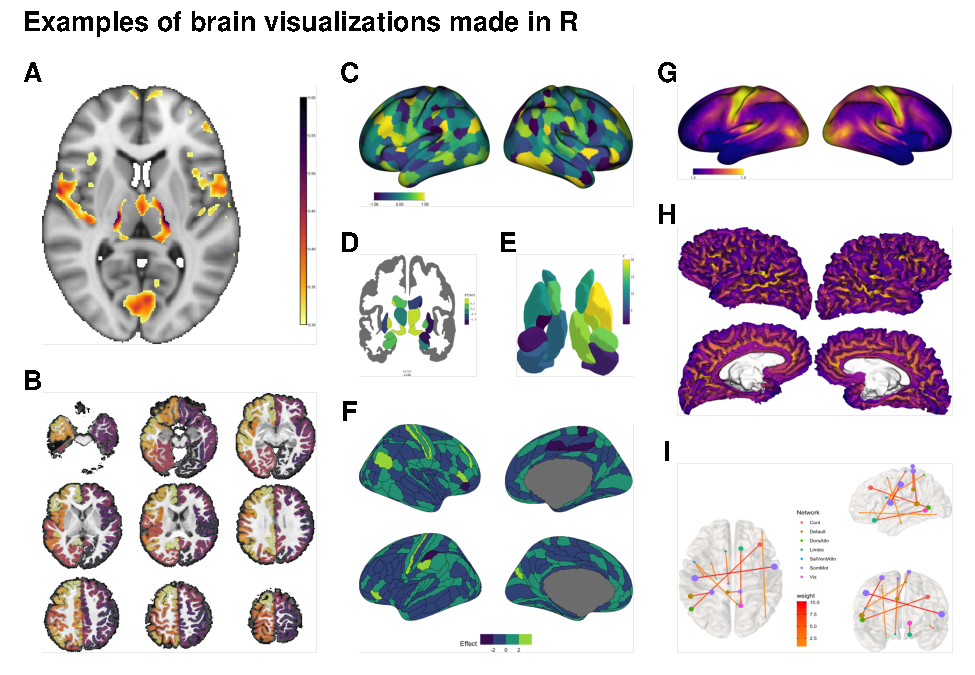
\includegraphics[width=0.8\linewidth,height=0.8\textheight]{manuscript_files/figure-latex/Figure1 -1} \end{center}

\emph{Figure 1. Examples of brain imaging visualization make in using different R-packages.} A) Voxel-based statistical map threshold and overlaid over a T1-weighted template data, with a single axial slice shown. Made using the the \texttt{ortho2} function from the \texttt{neurobase} package. B) A voxel-level cortical parcellation overlaid on T1-weighted MRI data shown in 9-slice axial orientation. Made using the \texttt{overlay} function from the \texttt{neurobase} package. C) A CIFTI format surface ROI atlas with a corresponding statistic assigned to each regions, with both hemispheres displayed on a inflated template surface in lateral view. Made using the \texttt{view\_xifti\_surface} from the \texttt{ciftiTools} package. D) A coronal cross-sectional rendering of subcortical structures where a statistical value has been assigned to each region. Made using the \texttt{aseg} atlas from the \texttt{ggseg} package. E) A 3D rendering of 9 bilateral subcortical regions where a statistical value has been assigned to each region. Made using the \texttt{aseg} atlas from the \texttt{ggseg3d} package. F) Medial and lateral views of a ROI atlas displayed on inflated template cortical surface where a statistical value has been assigned to each region. Made using the \texttt{glasser} atlas from the \texttt{ggsegGlasser} package, which was plotted using \texttt{ggseg}. G) Lateral view of a CIFTI format vertex-level data displayed on a inflated template surface. Made using the \texttt{view\_xifti\_surface} function from the \texttt{ciftiTools} package. H) Medial and lateral views of vertex-level data displayed on a individuals white matter surface. Made using the \texttt{vis.subject.morph.standard} function from the \texttt{fsbrain} package. I) A weighted and undirected graph plotted on top, left and front views of a template of a brain rendering. Made using the \texttt{brainconn} function from the \texttt{brainconn} package. All code used to compile this figure, as well as the contents of each panel are provided in the Supplement.

\end{landscape}

\hypertarget{voxel-level-visualizations.}{%
\subsection{Voxel-Level Visualizations.}\label{voxel-level-visualizations.}}

The \texttt{oro.nifti} and \texttt{neurobase} packages allow for the reading, writing, manipulation and visualization of voxel-level imaging data of either \emph{nifti}, \emph{analyze} or \emph{afni} formats. In particular, the \texttt{image}, \texttt{slice} and \texttt{ortho2} functions allow users to display the desired number of slices in the desired orientations, while also providing precise control over overlaid images, color scales, legend placement and other aesthetic settings (Fig 1A-B). Smoothing and re-sampling of images is sometimes required for visualization purposes, which can be achieved via the \texttt{ANTsR} or \texttt{fslr} packages.

\hypertarget{vertex-level-visualizations.}{%
\subsection{Vertex-Level Visualizations.}\label{vertex-level-visualizations.}}

The recently developed \texttt{fsbrain} package allows for the visualization of vertex-level and cortical ROI-level data which were derived using \emph{FreeSurfer}. The package contains many flexible functions for visualizing individual-level and group-level measures such as cortical thickness, volume or surface area (Fig 1F). In addition to producing publication-ready figures, the visualization functions can allow for visual quality control of large datasets processed using FreeSurfer. The package also comes with extensive guides and documentations to assist users (Schäfer \& Ecker, 2020).

CIFTI or `grey-ordinate' data is becoming a popular format for structural and functional imaging data, as it combines vertex-level data of the cortex with voxel-level data for the cerebellum and sub-cortex. In R, CIFTI data can now be read, visualized and manipulated using the well-documented \texttt{ciftiTools} package (Fig 1C,1G; Pham, Muschelli, \& Mejia, 2022). This package allows for both vertex-level visualization of the surface as well as voxel-level visualization of cerebellum and subcortex.

\hypertarget{roi-level-visualizations.}{%
\subsection{ROI-Level Visualizations.}\label{roi-level-visualizations.}}

Statistical parameters can be mapped onto discreet cortical and sub-cortical regions using the \texttt{ggseg} and \texttt{ggseg3d} packages (Mowinckel \& Vidal-Piñeiro, 2020). These packages flexibly generates aesthetic renderings of cortical, sub-cortical and white matter ROIs in 2D (Fig 1D,1F) and 3D (Fig 1E). Usually, ROI-level interpretations are dependent on a standardized atlas or parcellation scheme of the brain and accordingly, this package and its sister-packages (\texttt{ggsegExtra}) provide a large array of commonly used atlases and some functionality for users to contribute other atlases. Additionally, being part of the `Grammar of Graphics' framework (Wickham, 2016) allows for integration with packages such as \texttt{gganimate}, enabling users to animate and visualize dynamic changes in spatial and temporal statistics across ROIs. Notably, the \texttt{ciftiTools} package also provides functions to visualize surface and voxel-level ROIs for the cortex and sub-cortex respectively (Fig 1E), flexibly allowing CIFTI format atlases and ROIs to be displayed.

\hypertarget{edge-level-visualizations.}{%
\subsection{Edge-Level Visualizations.}\label{edge-level-visualizations.}}

Analyses which divide the brain into discrete regions and examine pair-wise dependencies between regional phenotypes are becoming increasingly common. Often the results of these dependency analyses are statistics relating to `edges' or links between any two regions. The package \texttt{brainconn} allows users to plot brain regions as nodes of a network graph, and dependencies between regions as edges of that graph, following a standardized coordinate space in both 2D and interactive 3D (Figure 1I). The graphs can be weighted, with the strength of the edges represented with color or line thickness, as well as directed, where arrows will be used in place of edges. This package comes with node coordinates corresponding to multiple commonly used atlases and contains functionality for users to easily enter their own custom atlas coordinates.

\hypertarget{limitations-and-functionality-gaps}{%
\section{Limitations and Functionality Gaps}\label{limitations-and-functionality-gaps}}

Most of the tools introduced above do not require a strong knowledge of programming, but there is still a steeper learning curve when compared to use a GUI. This is especially true when learning how to make fine adjustments to visual auxiliary such as legend placement, font size and multi-panel figure positioning, for the purpose of a publication-ready figure. While most code-based tools offer some control over these finer steps, there are differences between them in feature availability and usability. Relatedly, while some interactive image viewers which can be opened within an integrated development environment (e.g.~Muschelli, 2016), for quick and interactive viewing of single images, GUI tool can be faster and more practical.

Often cerebellar and brain-stem regions are not well represented in software (e.g.~Figure 1), potentially mirroring the cortico-centric sentiment that has prevailed in human neuroimaging research (Chin, Chang, \& Holmes, 2022). Likewise, custom non-cortical atlases such as non-standard subcortical atlas schemes are not yet straight forward, and usually require multiple functions and packages to visualize. Finally, some neuroimaging related data types, such as streamlines resulting from DWI-based tractography, are still not well represented in code-based visualization tools.

As can be seen in Table 1, there are usually multiple packages within each programming environment which are capable of visualizing each data type. While this provide choice for advanced users, it can also lead to confusion for novice users who may not be familiar with the nuanced differences between tools. Future work should continue to consolidate brain visualization methods into unified beginner-friendly code-based tools which are capable of plotting multiple data types.

\newpage

\hypertarget{references}{%
\section{References}\label{references}}

Poldrack, R. A., Baker, C. I., Durnez, J., Gorgolewski, K. J., Matthews, P. M., Munafò, M. R., \ldots{} \& Yarkoni, T. (2017). Scanning the horizon: towards transparent and reproducible neuroimaging research. Nature reviews neuroscience, 18(2), 115-126.

Steel, G. (2013, September 3). Publishing research without data is simply advertising, not science. Open Knowledge Foundation. \url{https://blog.okfn.org/2013/09/03/publishing-research-without-data-is-simply-advertising-not-science/}

The Comprehensive R Archive Network. (n.d.). Retrieved April 21, 2022, from \url{https://cran.r-project.org/}

Muschelli, J., Gherman, A., Fortin, J. P., Avants, B., Whitcher, B., Clayden, J. D., \ldots{} \& Crainiceanu, C. M. (2019). Neuroconductor: an R platform for medical imaging analysis. \emph{Biostatistics}, \emph{20}(2), 218-239.

Pham, D., Muschelli, J., \& Mejia, A. (2022). ciftiTools: A package for reading, writing, visualizing, and manipulating CIFTI files in R. \emph{NeuroImage}, 118877.

Mowinckel, A. M., \& Vidal-Piñeiro, D. (2020). Visualization of brain statistics with R packages ggseg and ggseg3d. \emph{Advances in Methods and Practices in Psychological Science}, \emph{3}(4), 466-483.

Huntenburg, J., Abraham, A., Loula, J., Liem, F., Dadi, K., \& Varoquaux, G. (2017). Loading and plotting of cortical surface representations in Nilearn. \emph{Research Ideas and Outcomes}, \emph{3}, e12342.

Wickham H. (2016). \emph{ggplot2: Elegant Graphics for Data Analysis.} Springer-Verlag New York. ISBN 978-3-319-24277-4, \url{https://ggplot2.tidyverse.org}.

Muschelli, J. (2016). \emph{papayar}. GitHub repository. \url{https://github.com/muschellij2/papayar}

David C. Van Essen, Stephen M. Smith, Deanna M. Barch, Timothy E.J. Behrens, Essa Yacoub, Kamil Ugurbil, for the WU-Minn HCP Consortium. (2013). The WU-Minn Human Connectome Project: An overview. NeuroImage 80(2013):62-79.

Sudlow, C., Gallacher, J., Allen, N., Beral, V., Burton, P., Danesh, J., \ldots{} \& Collins, R. (2015). UK biobank: an open access resource for identifying the causes of a wide range of complex diseases of middle and old age. PLoS medicine, 12(3), e1001779.

Esteban, O., Markiewicz, C. J., Blair, R. W., Moodie, C. A., Isik, A. I., Erramuzpe, A., \ldots{} \& Gorgolewski, K. J. (2019). fMRIPrep: a robust preprocessing pipeline for functional MRI. Nature methods, 16(1), 111-116.

Pernet, C., \& Madan, C. R. (2019). Data visualization for inference in tomographic brain imaging.

Code Ocean. (2021, October 27). Computational Research Platform on. Retrieved April 21, 2022, from \url{https://codeocean.com/}

Madan, C. R. (2015). Creating 3D visualizations of MRI data: A brief guide. F1000Research, 4.

Baker M. (2015). Social media: A network boost. Nature 518: 263--265. 10.1038/nj7538-263a

Lee J.-S. (2019). How to use Twitter to further your research career. Nature. 10.1038/d41586-019-00535-w

Li, Y., \& Xie, Y. (2020). Is a picture worth a thousand words? An empirical study of image content and social media engagement. Journal of Marketing Research, 57(1), 1-19.

Schäfer, T., \& Ecker, C. (2020). fsbrain: an R package for the visualization of structural neuroimaging data. bioRxiv.

Chin, R., Chang, S. W., \& Holmes, A. J. (2022). Beyond cortex: The evolution of the human brain. \emph{Psychological Review}.

\newpage

\hypertarget{supplement-code-used-to-generate-figures}{%
\section{Supplement (Code used to generate Figures)}\label{supplement-code-used-to-generate-figures}}

\singlespacing

\begin{Shaded}
\begin{Highlighting}[]
\CommentTok{\#Figure 1A (Voxel)}

\FunctionTok{library}\NormalTok{(neurobase)}

\CommentTok{\#Load in a nifti (.nii.gz) file of a standardized template so use as a background. }
\NormalTok{template }\OtherTok{\textless{}{-}} \FunctionTok{readnii}\NormalTok{(}\StringTok{\textquotesingle{}data/MNI152\_T1\_1mm\_brain.nii.gz\textquotesingle{}}\NormalTok{) }\CommentTok{\#load the nifti file into R}

\CommentTok{\#Load in a nifti (.nii.gz) file of the statistic you wanted of overlay, with the same dimensions as the template.  }
\NormalTok{effect }\OtherTok{\textless{}{-}} \FunctionTok{readnii}\NormalTok{(}\StringTok{"data/MNI152\_effect\_size.nii.gz"}\NormalTok{) }

\CommentTok{\#Threshold the statistic map so only values about a specified amount are displayed}
\NormalTok{effect[effect}\SpecialCharTok{\textless{}}\FloatTok{0.3}\NormalTok{] }\OtherTok{\textless{}{-}} \ConstantTok{NA} 

\CommentTok{\#Set the breaks/intervals you want on the color bar (e.g. from .3 to .6, by intervals of 0.005)}
\NormalTok{breaks }\OtherTok{=} \FunctionTok{seq}\NormalTok{(.}\DecValTok{3}\NormalTok{,.}\DecValTok{6}\NormalTok{, }\AttributeTok{by=}\FloatTok{0.005}\NormalTok{)}

\CommentTok{\#[Optional] If you want to output the figure as a .png, open a png image device}
\FunctionTok{png}\NormalTok{(}\StringTok{"data/fig1a.png"}\NormalTok{) }

\CommentTok{\#Use the ortho2 function from the neurobase package to make the figure}
\FunctionTok{ortho2}\NormalTok{(}\AttributeTok{x =}\NormalTok{ template,   }\CommentTok{\#Specify the background template}
       \AttributeTok{y =}\NormalTok{ effect,     }\CommentTok{\#Specify the effect you want to overlay on the template}
       \AttributeTok{crosshairs =}\NormalTok{ F, }\CommentTok{\#Remove the cross{-}hairs}
       \AttributeTok{bg =} \StringTok{"white"}\NormalTok{,   }\CommentTok{\#Make the background white }
       \AttributeTok{NA.x =}\NormalTok{ T,       }\CommentTok{\#Do not display NA values}
       \AttributeTok{col.y=} \FunctionTok{rev}\NormalTok{(viridis}\SpecialCharTok{::}\FunctionTok{inferno}\NormalTok{(}\AttributeTok{n =} \DecValTok{500}\NormalTok{)), }\CommentTok{\#Select the color scale. In this case I have used the inferno scale from the viridis package. }
       \AttributeTok{xyz =} \FunctionTok{c}\NormalTok{(}\DecValTok{70}\NormalTok{,}\DecValTok{50}\NormalTok{,}\DecValTok{80}\NormalTok{), }\CommentTok{\#set the x y \& z slice you want to visualize}
       \AttributeTok{useRaster =}\NormalTok{ T,     }\CommentTok{\#Sometimes using Raster makes for clearer plots}
       \AttributeTok{ycolorbar =} \ConstantTok{TRUE}\NormalTok{,  }\CommentTok{\#Add a color bar}
       \AttributeTok{mfrow =} \FunctionTok{c}\NormalTok{(}\DecValTok{1}\NormalTok{,}\DecValTok{1}\NormalTok{)) }\SpecialCharTok{+}  \CommentTok{\#layout of brain views (for this figure, we just want a axial view)}
  \FunctionTok{colorbar}\NormalTok{(breaks, }\AttributeTok{col =} \FunctionTok{rev}\NormalTok{(viridis}\SpecialCharTok{::}\FunctionTok{inferno}\NormalTok{(}\AttributeTok{n=}\FunctionTok{length}\NormalTok{(breaks)}\SpecialCharTok{{-}}\DecValTok{1}\NormalTok{)), }\CommentTok{\#add a color bar with same color scale }
           \AttributeTok{text.col =} \StringTok{"black"}\NormalTok{, }\AttributeTok{labels =} \ConstantTok{TRUE}\NormalTok{, }\AttributeTok{maxleft =} \FloatTok{0.95}\NormalTok{)  }\CommentTok{\#Set the specifications for the color bar}

\FunctionTok{dev.off}\NormalTok{()}
\end{Highlighting}
\end{Shaded}

\begin{Shaded}
\begin{Highlighting}[]
\CommentTok{\#Figure 1B (Voxel)}

\FunctionTok{library}\NormalTok{(neurobase)}
\FunctionTok{library}\NormalTok{(scales)}

\CommentTok{\#Load in a nifti (.nii.gz) file to use as a background. }
\NormalTok{t1 }\OtherTok{\textless{}{-}} \FunctionTok{readnii}\NormalTok{(}\StringTok{\textquotesingle{}data/sub{-}001\_\_t1\_warped.nii.gz\textquotesingle{}}\NormalTok{) }

\CommentTok{\#Load in a nifti (.nii.gz) file to use as a overlay. }
\NormalTok{atlas }\OtherTok{\textless{}{-}}  \FunctionTok{readnii}\NormalTok{(}\StringTok{\textquotesingle{}data/sub{-}001\_schaefer300n7\_aseg\_to\_dwispace\_gm\_rois.nii.gz\textquotesingle{}}\NormalTok{)}

\FunctionTok{png}\NormalTok{(}\StringTok{\textquotesingle{}data/fig1b.png\textquotesingle{}}\NormalTok{)}
\FunctionTok{overlay}\NormalTok{(}\AttributeTok{x=}\FunctionTok{robust\_window}\NormalTok{(t1), }\AttributeTok{y=}\NormalTok{atlas, }
        \AttributeTok{plot.type =} \StringTok{"single"}\NormalTok{, }
        \AttributeTok{z=}\FunctionTok{c}\NormalTok{(}\FunctionTok{seq}\NormalTok{(}\DecValTok{30}\NormalTok{,}\DecValTok{110}\NormalTok{,}\DecValTok{10}\NormalTok{)), }
        \AttributeTok{col.y =}  \FunctionTok{alpha}\NormalTok{(viridis}\SpecialCharTok{::}\FunctionTok{inferno}\NormalTok{(}\DecValTok{300}\NormalTok{), }\FloatTok{0.6}\NormalTok{),}
        \AttributeTok{plane =} \StringTok{"axial"}\NormalTok{,  }
        \AttributeTok{useRaster =}\NormalTok{ T, }
        \AttributeTok{bg =} \StringTok{"white"}\NormalTok{,}
        \AttributeTok{NA.x=}\NormalTok{T, }
        \AttributeTok{zlim.y =}\FunctionTok{c}\NormalTok{(}\DecValTok{1}\NormalTok{,}\DecValTok{300}\NormalTok{))}
\FunctionTok{dev.off}\NormalTok{()}
\end{Highlighting}
\end{Shaded}

\begin{Shaded}
\begin{Highlighting}[]
\CommentTok{\#vertex 1}
\CommentTok{\#Figure 1C}
\FunctionTok{library}\NormalTok{(rgl)}
\FunctionTok{library}\NormalTok{(ggplot2)}
\CommentTok{\# Load the package and point to the Connectome Workbench}
\FunctionTok{library}\NormalTok{(ciftiTools)}

\CommentTok{\#Need connectome workbench to use ciftiTools {-} set path below}
\FunctionTok{ciftiTools.setOption}\NormalTok{(}\StringTok{"wb\_path"}\NormalTok{, }\StringTok{"/Applications/workbench/"}\NormalTok{)}

\CommentTok{\# Read in CIFTI file}
\NormalTok{cifti\_fname }\OtherTok{\textless{}{-}}\NormalTok{ ciftiTools}\SpecialCharTok{::}\FunctionTok{ciftiTools.files}\NormalTok{()}\SpecialCharTok{$}\NormalTok{cifti[}\StringTok{"dtseries"}\NormalTok{]}
\NormalTok{surfL\_fname }\OtherTok{\textless{}{-}} \FunctionTok{ciftiTools.files}\NormalTok{()}\SpecialCharTok{$}\NormalTok{surf[}\StringTok{"left"}\NormalTok{]}
\NormalTok{surfR\_fname }\OtherTok{\textless{}{-}} \FunctionTok{ciftiTools.files}\NormalTok{()}\SpecialCharTok{$}\NormalTok{surf[}\StringTok{"right"}\NormalTok{]}

\NormalTok{cii }\OtherTok{\textless{}{-}} \FunctionTok{read\_cifti}\NormalTok{(}
\NormalTok{  cifti\_fname, }\AttributeTok{brainstructures=}\StringTok{"all"}\NormalTok{, }
  \AttributeTok{surfL\_fname=}\NormalTok{surfL\_fname,}
  \AttributeTok{surfR\_fname=}\NormalTok{surfR\_fname)}

\CommentTok{\#Plot cifti surface}
\FunctionTok{view\_xifti\_surface}\NormalTok{(cii, }
                   \AttributeTok{hemisphere =} \StringTok{"both"}\NormalTok{, }
                   \AttributeTok{view =} \StringTok{"lateral"}\NormalTok{, }
                   \AttributeTok{idx =} \DecValTok{1}\NormalTok{,}
                   \AttributeTok{colors =}\NormalTok{ viridis}\SpecialCharTok{::}\FunctionTok{plasma}\NormalTok{(}\AttributeTok{n =} \DecValTok{100}\NormalTok{),}
                   \AttributeTok{zlim =} \FunctionTok{c}\NormalTok{(}\FloatTok{1.2}\NormalTok{,}\FloatTok{1.5}\NormalTok{),  }
                   \AttributeTok{legend\_embed =}\NormalTok{ T,}
                   \AttributeTok{cex.title =} \DecValTok{2}\NormalTok{)}



\FunctionTok{rgl.snapshot}\NormalTok{(}\StringTok{"data/fig1c.png"}\NormalTok{)}
\FunctionTok{rgl.close}\NormalTok{()}
\end{Highlighting}
\end{Shaded}

\begin{Shaded}
\begin{Highlighting}[]
\CommentTok{\#Vertex 2}
\CommentTok{\#Figure 1X {-} Remove white space}


\FunctionTok{library}\NormalTok{(fsbrain)}
\FunctionTok{library}\NormalTok{(rgl)}

\CommentTok{\#download\_optional\_data()}
\CommentTok{\#download\_fsaverage(accept\_freesurfer\_license = TRUE)}

\NormalTok{subjects\_dir }\OtherTok{\textless{}{-}} \FunctionTok{get\_optional\_data\_filepath}\NormalTok{(}\StringTok{"subjects\_dir"}\NormalTok{)}

\NormalTok{subject\_id }\OtherTok{\textless{}{-}} \StringTok{\textquotesingle{}subject1\textquotesingle{}} 

\NormalTok{colourmap }\OtherTok{\textless{}{-}} \FunctionTok{colorRampPalette}\NormalTok{(viridis}\SpecialCharTok{::}\FunctionTok{plasma}\NormalTok{(}\AttributeTok{n =} \DecValTok{1000}\NormalTok{))}
\FunctionTok{fsbrain.set.default.figsize}\NormalTok{(}\DecValTok{700}\NormalTok{, }\DecValTok{700}\NormalTok{);}

\NormalTok{brain }\OtherTok{=} \FunctionTok{vis.subject.morph.native}\NormalTok{(subjects\_dir, }
\NormalTok{                                subject\_id, }\StringTok{\textquotesingle{}sulc\textquotesingle{}}\NormalTok{, }
                                \AttributeTok{cortex\_only =}\NormalTok{ T, }
                                \AttributeTok{views=}\ConstantTok{NULL}\NormalTok{, }
                                \AttributeTok{draw\_colorbar =} \ConstantTok{FALSE}\NormalTok{,}
                                \AttributeTok{makecmap\_options =} \FunctionTok{list}\NormalTok{(}\StringTok{\textquotesingle{}colFn\textquotesingle{}}\OtherTok{=}\NormalTok{colourmap))}

\NormalTok{img }\OtherTok{=} \FunctionTok{export}\NormalTok{(brain, }\AttributeTok{draw\_colorbar =} \ConstantTok{FALSE}\NormalTok{, }\AttributeTok{output\_img =} \StringTok{"data/fig1d.png"}\NormalTok{)}
\end{Highlighting}
\end{Shaded}

\begin{Shaded}
\begin{Highlighting}[]
\CommentTok{\#ROI1 }
\CommentTok{\#Figure 1e }
\FunctionTok{library}\NormalTok{(ciftiTools)}
\NormalTok{parc }\OtherTok{\textless{}{-}} \FunctionTok{load\_parc}\NormalTok{(}\StringTok{"Yeo\_7"}\NormalTok{)}
\FunctionTok{view\_xifti\_surface}\NormalTok{(parc,  }
                   \AttributeTok{legend\_embed =}\NormalTok{ T,}
                   \AttributeTok{hemisphere =} \StringTok{"right"}\NormalTok{)}

\FunctionTok{rgl.snapshot}\NormalTok{(}\StringTok{"data/fig1e.png"}\NormalTok{)}

\FunctionTok{rgl.close}\NormalTok{()}
\end{Highlighting}
\end{Shaded}

\begin{Shaded}
\begin{Highlighting}[]
\CommentTok{\#ROI1 }
\CommentTok{\#Figure 1X {-} combine with previous figure}

\FunctionTok{set.seed}\NormalTok{(}\DecValTok{1993}\NormalTok{) }\CommentTok{\#set a random seed (good practice for reproducibility)}

\NormalTok{parc }\OtherTok{\textless{}{-}} \FunctionTok{load\_parc}\NormalTok{(}\StringTok{"Schaefer\_400"}\NormalTok{)}

\NormalTok{ramdom\_metric }\OtherTok{\textless{}{-}} \FunctionTok{rnorm}\NormalTok{(}\DecValTok{400}\NormalTok{)}

\NormalTok{cii }\OtherTok{\textless{}{-}} \FunctionTok{move\_from\_mwall}\NormalTok{(cii, }\ConstantTok{NA}\NormalTok{)}

\NormalTok{parc\_vec }\OtherTok{\textless{}{-}} \FunctionTok{c}\NormalTok{(}\FunctionTok{as.matrix}\NormalTok{(parc))}

\NormalTok{xii\_metric }\OtherTok{\textless{}{-}} \FunctionTok{c}\NormalTok{(}\ConstantTok{NA}\NormalTok{, ramdom\_metric)[parc\_vec }\SpecialCharTok{+} \DecValTok{1}\NormalTok{]}

\NormalTok{xii1 }\OtherTok{\textless{}{-}} \FunctionTok{select\_xifti}\NormalTok{(cii, }\DecValTok{1}\NormalTok{)}

\NormalTok{xii\_metric }\OtherTok{\textless{}{-}} \FunctionTok{newdata\_xifti}\NormalTok{(xii1, xii\_metric)}

\NormalTok{plot2 }\OtherTok{\textless{}{-}} \FunctionTok{view\_xifti\_surface}\NormalTok{(xii\_metric, }
                            \AttributeTok{colors =}\NormalTok{ viridis}\SpecialCharTok{::}\FunctionTok{viridis}\NormalTok{(}\AttributeTok{n =} \DecValTok{400}\NormalTok{), }
                            \AttributeTok{borders =} \StringTok{"black"}\NormalTok{, }
                            \AttributeTok{hemisphere =} \StringTok{"both"}\NormalTok{,}
                            \AttributeTok{view =} \StringTok{\textquotesingle{}lateral\textquotesingle{}}\NormalTok{)}

\FunctionTok{rgl.snapshot}\NormalTok{(}\StringTok{"data/fig1f.png"}\NormalTok{)}

\FunctionTok{rgl.close}\NormalTok{()}
\end{Highlighting}
\end{Shaded}

\begin{Shaded}
\begin{Highlighting}[]
\CommentTok{\#ROI2}

\CommentTok{\#devtools::install\_github("LCBC{-}UiO/ggsegGlasser")}
\FunctionTok{library}\NormalTok{(ggseg)}
\FunctionTok{library}\NormalTok{(ggplot2)}
\FunctionTok{library}\NormalTok{(ggsegGlasser)}

\FunctionTok{set.seed}\NormalTok{(}\DecValTok{1993}\NormalTok{) }\CommentTok{\#set a random seed (good practice for reproducibility)}


\NormalTok{base\_atlas }\OtherTok{\textless{}{-}} \FunctionTok{as.data.frame}\NormalTok{(}\FunctionTok{na.omit}\NormalTok{(}\FunctionTok{cbind}\NormalTok{(glasser}\SpecialCharTok{$}\NormalTok{data}\SpecialCharTok{$}\NormalTok{region, glasser}\SpecialCharTok{$}\NormalTok{data}\SpecialCharTok{$}\NormalTok{hemi)))}

\FunctionTok{colnames}\NormalTok{(base\_atlas) }\OtherTok{\textless{}{-}} \FunctionTok{c}\NormalTok{(}\StringTok{"region"}\NormalTok{, }\StringTok{"hemi"}\NormalTok{)}

\NormalTok{Effect }\OtherTok{\textless{}{-}} \FunctionTok{rnorm}\NormalTok{(}\FunctionTok{dim}\NormalTok{(base\_atlas)[}\DecValTok{1}\NormalTok{]) }\CommentTok{\#generate a random numbers for each roi in the atlas}

\NormalTok{base\_atlas }\OtherTok{\textless{}{-}} \FunctionTok{cbind}\NormalTok{(Effect, base\_atlas)}


\NormalTok{cortex }\OtherTok{\textless{}{-}} \FunctionTok{ggseg}\NormalTok{(}\AttributeTok{atlas =}\NormalTok{ glasser,}
                \AttributeTok{.data =}\NormalTok{ base\_atlas,}
                \AttributeTok{mapping=}\FunctionTok{aes}\NormalTok{(}\AttributeTok{fill=}\NormalTok{Effect), }
                \AttributeTok{position=}\StringTok{"stacked"}\NormalTok{,}
                \AttributeTok{colour=}\StringTok{"black"}\NormalTok{,}
                \AttributeTok{size=}\NormalTok{.}\DecValTok{2}\NormalTok{,}
                \AttributeTok{show.legend =}\NormalTok{ T,}
                \AttributeTok{plot.background =} \StringTok{"white"}\NormalTok{) }\SpecialCharTok{+}
  \FunctionTok{scale\_fill\_viridis\_b}\NormalTok{() }\SpecialCharTok{+} 
   \FunctionTok{theme\_void}\NormalTok{() }\SpecialCharTok{+}
    \FunctionTok{theme}\NormalTok{(}\AttributeTok{legend.position =} \StringTok{"bottom"}\NormalTok{)}

\NormalTok{sub\_base\_atlas }\OtherTok{\textless{}{-}} \FunctionTok{as.data.frame}\NormalTok{(}\FunctionTok{na.omit}\NormalTok{(}\FunctionTok{cbind}\NormalTok{(aseg}\SpecialCharTok{$}\NormalTok{data}\SpecialCharTok{$}\NormalTok{region, aseg}\SpecialCharTok{$}\NormalTok{data}\SpecialCharTok{$}\NormalTok{hemi)))}

\FunctionTok{colnames}\NormalTok{(sub\_base\_atlas) }\OtherTok{\textless{}{-}} \FunctionTok{c}\NormalTok{(}\StringTok{"region"}\NormalTok{, }\StringTok{"hemi"}\NormalTok{)}

\NormalTok{Effect }\OtherTok{\textless{}{-}} \FunctionTok{rnorm}\NormalTok{(}\FunctionTok{dim}\NormalTok{(sub\_base\_atlas)[}\DecValTok{1}\NormalTok{])}

\NormalTok{sub\_base\_atlas }\OtherTok{\textless{}{-}} \FunctionTok{cbind}\NormalTok{(Effect, sub\_base\_atlas)}

\NormalTok{subcortex }\OtherTok{\textless{}{-}} \FunctionTok{ggseg}\NormalTok{(}\AttributeTok{atlas =}\NormalTok{ aseg,}
                   \AttributeTok{.data =}\NormalTok{ sub\_base\_atlas,}
                   \AttributeTok{mapping=}\FunctionTok{aes}\NormalTok{(}\AttributeTok{fill=}\NormalTok{Effect), }
                   \AttributeTok{position =} \StringTok{"dispersed"}\NormalTok{,}
                   \AttributeTok{colour=}\StringTok{"black"}\NormalTok{,}
                   \AttributeTok{hemi =}\FunctionTok{c}\NormalTok{(}\StringTok{\textquotesingle{}left\textquotesingle{}}\NormalTok{, }\StringTok{\textquotesingle{}right\textquotesingle{}}\NormalTok{),}
                   \AttributeTok{size=}\NormalTok{.}\DecValTok{2}\NormalTok{,}
                   \AttributeTok{show.legend =}\NormalTok{ T, }
                   \AttributeTok{plot.background =} \StringTok{"white"}\NormalTok{) }\SpecialCharTok{+} 
  \FunctionTok{scale\_fill\_viridis\_b}\NormalTok{() }

\FunctionTok{ggsave}\NormalTok{(}\AttributeTok{filename =} \StringTok{\textquotesingle{}data/fig1g1.png\textquotesingle{}}\NormalTok{, }\AttributeTok{plot =}\NormalTok{ cortex, }\AttributeTok{device =} \StringTok{\textquotesingle{}png\textquotesingle{}}\NormalTok{, }\AttributeTok{bg =} \StringTok{\textquotesingle{}white\textquotesingle{}}\NormalTok{)}
\FunctionTok{ggsave}\NormalTok{(}\AttributeTok{filename =} \StringTok{\textquotesingle{}data/fig1g2.png\textquotesingle{}}\NormalTok{, }\AttributeTok{plot =}\NormalTok{ subcortex, }\AttributeTok{device =} \StringTok{\textquotesingle{}png\textquotesingle{}}\NormalTok{, }\AttributeTok{bg =} \StringTok{\textquotesingle{}white\textquotesingle{}}\NormalTok{)}
\end{Highlighting}
\end{Shaded}

\begin{Shaded}
\begin{Highlighting}[]
\NormalTok{make\_ggseg3d }\OtherTok{\textless{}{-}} \ControlFlowTok{function}\NormalTok{(attribute, }
                         \AttributeTok{colour.pal =} \FunctionTok{c}\NormalTok{(}\StringTok{"light yellow"}\NormalTok{,}
                                        \StringTok{"orange"}\NormalTok{,}
                                        \StringTok{"red"}\NormalTok{,}
                                        \StringTok{"dark red"}\NormalTok{), }
                         \AttributeTok{hide.colourbar=}\ConstantTok{FALSE}\NormalTok{, }
                         \AttributeTok{output.png=}\ConstantTok{FALSE}\NormalTok{, }
                         \AttributeTok{file.name=}\StringTok{"ggseg\_3d.png"}\NormalTok{) \{}
  \CommentTok{\# Inputs: }
  \CommentTok{\#\textquotesingle{} attribute = This must be a numeric vector in this: Left{-}Thalamus, Left{-}Caudate, Left{-}Putamen, Left{-}Pallidum Left{-}Hippocampus, Left{-}Amygdala, Left{-}Accumbens{-}area, Right{-}Thalamus{-}Proper, Right{-}Caudate, Right{-}Putamen, Right{-}Pallidum, Right{-}Hippocampus, Right{-}Amygdala, Right{-}Accumbens{-}area}
  
  \FunctionTok{library}\NormalTok{(ggseg3d)}
  \FunctionTok{library}\NormalTok{(tidyr)}
  \FunctionTok{library}\NormalTok{(dplyr)}
  \CommentTok{\#remove(aseg\_3d)}
\NormalTok{  aseg\_3d }\OtherTok{\textless{}{-}}\NormalTok{ aseg\_3d}
\NormalTok{  aseg\_3d }\OtherTok{\textless{}{-}}\NormalTok{ tidyr}\SpecialCharTok{::}\FunctionTok{unnest}\NormalTok{(aseg\_3d, }\AttributeTok{cols =} \FunctionTok{c}\NormalTok{(ggseg\_3d))}
  
\NormalTok{  attribute.ggseg3d }\OtherTok{\textless{}{-}} \FunctionTok{c}\NormalTok{(}\FunctionTok{rep}\NormalTok{(}\ConstantTok{NA}\NormalTok{, }\DecValTok{4}\NormalTok{), attribute[}\DecValTok{1}\SpecialCharTok{:}\DecValTok{4}\NormalTok{], }\FunctionTok{rep}\NormalTok{(}\ConstantTok{NA}\NormalTok{, }\DecValTok{3}\NormalTok{), attribute[}\DecValTok{5}\SpecialCharTok{:}\DecValTok{7}\NormalTok{],}
                         \FunctionTok{rep}\NormalTok{(}\ConstantTok{NA}\NormalTok{, }\DecValTok{5}\NormalTok{), attribute[}\DecValTok{8}\SpecialCharTok{:}\DecValTok{14}\NormalTok{],  }\FunctionTok{rep}\NormalTok{(}\ConstantTok{NA}\NormalTok{, }\DecValTok{6}\NormalTok{))}
  
\NormalTok{  data }\OtherTok{\textless{}{-}}\NormalTok{ dplyr}\SpecialCharTok{::}\FunctionTok{mutate}\NormalTok{(aseg\_3d, }\AttributeTok{attribute =}\NormalTok{  attribute.ggseg3d)}
  \CommentTok{\#remove NA regions}
\NormalTok{  aseg\_3d[}\FunctionTok{which}\NormalTok{(}\FunctionTok{is.na}\NormalTok{(data}\SpecialCharTok{$}\NormalTok{attribute)),] }\OtherTok{\textless{}{-}} \ConstantTok{NA}
\NormalTok{  aseg\_3d }\OtherTok{\textless{}{-}}\NormalTok{ tidyr}\SpecialCharTok{::}\FunctionTok{drop\_na}\NormalTok{(aseg\_3d)}
  
\NormalTok{  data[}\FunctionTok{which}\NormalTok{(}\FunctionTok{is.na}\NormalTok{(data}\SpecialCharTok{$}\NormalTok{attribute)),] }\OtherTok{\textless{}{-}} \ConstantTok{NA}
\NormalTok{  data }\OtherTok{\textless{}{-}}\NormalTok{ tidyr}\SpecialCharTok{::}\FunctionTok{drop\_na}\NormalTok{(data)}
\NormalTok{  data}\SpecialCharTok{$}\NormalTok{attribute[data}\SpecialCharTok{$}\NormalTok{attribute}\SpecialCharTok{==}\DecValTok{0}\NormalTok{]}\OtherTok{\textless{}{-}}\ConstantTok{NA} \CommentTok{\#make 0 valus NA so they are set as grey in ggseg3d}
  
\NormalTok{  scene}\OtherTok{=}\FunctionTok{list}\NormalTok{(}\AttributeTok{camera =} \FunctionTok{list}\NormalTok{(}\AttributeTok{eye =} \FunctionTok{list}\NormalTok{(}\AttributeTok{x =} \DecValTok{0}\NormalTok{, }\AttributeTok{y =} \DecValTok{1}\NormalTok{, }\AttributeTok{z =} \SpecialCharTok{{-}}\FloatTok{2.25}\NormalTok{)),}
             \AttributeTok{aspectratio =} \FunctionTok{list}\NormalTok{(}\AttributeTok{x=}\FloatTok{1.6}\NormalTok{,}\AttributeTok{y=}\FloatTok{1.6}\NormalTok{,}\AttributeTok{z=}\FloatTok{1.6}\NormalTok{))}
  
  
\NormalTok{  plot }\OtherTok{\textless{}{-}}\NormalTok{ ggseg3d}\SpecialCharTok{::}\FunctionTok{ggseg3d}\NormalTok{(}\AttributeTok{.data =}\NormalTok{ data, }
                           \AttributeTok{atlas =}\NormalTok{ aseg\_3d, }
                           \AttributeTok{colour =} \StringTok{"attribute"}\NormalTok{, }
                           \AttributeTok{text =} \StringTok{"attribute"}\NormalTok{,}
                           \AttributeTok{palette =}\NormalTok{ colour.pal)}
\NormalTok{  plot }\OtherTok{\textless{}{-}} \FunctionTok{remove\_axes}\NormalTok{(plot)}
\NormalTok{  plot }\OtherTok{\textless{}{-}}\NormalTok{ plotly}\SpecialCharTok{::}\FunctionTok{layout}\NormalTok{(plot, }
                         \AttributeTok{scene =}\NormalTok{ scene, }
                         \AttributeTok{width =} \DecValTok{600}\NormalTok{, }\AttributeTok{height =} \DecValTok{600}\NormalTok{) }
  
  \ControlFlowTok{if}\NormalTok{(hide.colourbar}\SpecialCharTok{==}\ConstantTok{TRUE}\NormalTok{)\{}
\NormalTok{    plot }\OtherTok{\textless{}{-}}\NormalTok{ plotly}\SpecialCharTok{::}\FunctionTok{hide\_colorbar}\NormalTok{(plot)}
\NormalTok{  \}}
  
  \ControlFlowTok{if}\NormalTok{( output.png}\SpecialCharTok{==}\ConstantTok{TRUE}\NormalTok{)\{}
\NormalTok{    plotly}\SpecialCharTok{::}\FunctionTok{orca}\NormalTok{(plot, }\AttributeTok{file =}\NormalTok{  file.name)}
\NormalTok{  \}}
  
  \FunctionTok{return}\NormalTok{(plot)}
  
\NormalTok{\}}

\FunctionTok{set.seed}\NormalTok{(}\DecValTok{1993}\NormalTok{)}
\NormalTok{volume }\OtherTok{\textless{}{-}} \FunctionTok{sample}\NormalTok{(}\DecValTok{1}\SpecialCharTok{:}\DecValTok{20}\NormalTok{, }\DecValTok{14}\NormalTok{) }\CommentTok{\#randomly generated data for 14 structures}
\FunctionTok{make\_ggseg3d}\NormalTok{(volume, }
             \AttributeTok{colour.pal =}\NormalTok{ viridis}\SpecialCharTok{::}\FunctionTok{viridis}\NormalTok{(}\AttributeTok{n=}\FunctionTok{length}\NormalTok{(volume)), }
             \AttributeTok{output.png =}\NormalTok{ T, }\AttributeTok{file.name =} \StringTok{"data/fig1g3.png"}\NormalTok{)}
\end{Highlighting}
\end{Shaded}

\begin{Shaded}
\begin{Highlighting}[]
\CommentTok{\#Edge (also add 3d version)}
\CommentTok{\#Fig1X}

\CommentTok{\#devtools::install\_github("sidchop/brainconn")}
\FunctionTok{library}\NormalTok{(brainconn)}

\NormalTok{conmat }\OtherTok{\textless{}{-}}\NormalTok{ example\_weighted\_undirected}
\NormalTok{degree }\OtherTok{\textless{}{-}} \FunctionTok{rowSums}\NormalTok{(conmat)[}\FunctionTok{which}\NormalTok{(}\FunctionTok{rowSums}\NormalTok{(conmat)}\SpecialCharTok{!=}\DecValTok{0}\NormalTok{)]}

\FunctionTok{brainconn}\NormalTok{(}\AttributeTok{atlas =}\StringTok{"schaefer300\_n7"}\NormalTok{, }
                   \AttributeTok{conmat=}\NormalTok{conmat, }
                   \AttributeTok{node.size =}\NormalTok{ degree}\SpecialCharTok{/}\DecValTok{2}\NormalTok{,}
                   \AttributeTok{view=}\StringTok{"top"}\NormalTok{, }
                   \AttributeTok{edge.color.weighted =}\NormalTok{ T,}
                   \AttributeTok{background.alpha =} \FloatTok{0.8}\NormalTok{, }
                   \AttributeTok{show.legend =}\NormalTok{ F, }
                   \AttributeTok{edge.color =} \FunctionTok{scale\_edge\_colour\_viridis}\NormalTok{()) }



\FunctionTok{ggsave}\NormalTok{(}\AttributeTok{filename =} \StringTok{\textquotesingle{}data/fig1h.png\textquotesingle{}}\NormalTok{, }
       \AttributeTok{plot =}\NormalTok{ fig1h, }
       \AttributeTok{device =} \StringTok{\textquotesingle{}png\textquotesingle{}}\NormalTok{,}
       \AttributeTok{bg =} \StringTok{\textquotesingle{}white\textquotesingle{}}\NormalTok{,}
       \AttributeTok{height =} \DecValTok{7}\NormalTok{, }
       \AttributeTok{units =} \StringTok{"in"}\NormalTok{)}


\FunctionTok{brainconn3D}\NormalTok{(}\AttributeTok{atlas =}\StringTok{"schaefer300\_n7"}\NormalTok{, }
            \AttributeTok{conmat=}\NormalTok{conmat,}
            \AttributeTok{show.legend =}\NormalTok{ F)}
\end{Highlighting}
\end{Shaded}


\bibliographystyle{unsrt}
\bibliography{}


\end{document}
